\documentclass[conference]{IEEEtran}
\IEEEoverridecommandlockouts
% The preceding line is only needed to identify funding in the first footnote. If that is unneeded, please comment it out.
\usepackage{cite}
\usepackage{amsmath,amssymb,amsfonts}
\usepackage{algorithmic}
\usepackage{graphicx}
\usepackage{textcomp}
\usepackage{xcolor}
\usepackage{hyperref}
\usepackage{caption}
\usepackage{subcaption}

\def\BibTeX{{\rm B\kern-.05em{\sc i\kern-.025em b}\kern-.08em
    T\kern-.1667em\lower.7ex\hbox{E}\kern-.125emX}}

\begin{document}

\title{Degradable Objects : An Application To A Distributed Data Store}

\author{\IEEEauthorblockN{Adam CHADER}
\IEEEauthorblockA{\textit{PDS track, Master of Computer Science} \\
\textit{Institut Polytechnique de Paris}\\
Palaiseau, France \\
adam.chader@telecom-paris.fr}
}

\maketitle

\begin{abstract}
Ceci est un abstract
\end{abstract}

\begin{IEEEkeywords}
Concurrent programming, parallel programming, performance, databases
\end{IEEEkeywords}

\section{Introduction}
This paper is the report of a research project realised for the Parallel And Distributed Systems master at \textit{Institut Polytechnique de Paris}. It describes the work that I realised to apply degradable data structures to Apache Ignite \cite{ignite}, a distributed data store, to improve its performance and scalability.

\subsection{Context}
Up until the begnining of the 21\textsuperscript{st} Century, there had existed a simple rule that could be used to predict the performances of computers. This is known as Moore's Law (Fig.~\ref{moore}). This law states that every two year, the number of transistors would double on chips. This rule could be used quite flawlessly to predict the speed of software, as there is a direct correlation between the speed of sequential programs and the frequency of CPUs. However, in recent years, several issues have surfaced regarding these assumptions : Firstly, we seem to have reached the minimum physical size of a transistor at around 5 nanometer ; secondly, the frequency that can be reached by craming all these transistors in a single CPU core is too high to be dissipated by current means \cite{moore}. As of today, it is extremely complicated and costly to significantly increase the clock speed of a single core. The solution that was found is to put multiple CPU cores in a single machine. The total number of clock cycle per second should continue increasing, while the heat would remain manageable. Intuitively, this solution is perfect : by having two cores instead of one, we could double the total frequency of the CPU, and thus double the speed of software. This is what we call \textit{linear scalability}, and it is still just a dream. There are many reason as to why it is impossible to achieve linear scalability, but they all boil down to the same issue : in order to make the most out of several CPU cores, we need to have them working at the same time. It is possible when the tasks are perfectly parallelisable, but this almost never happens when we want the cores working together. Programs need to access variables in memory, and accessing them in parallel can cause conflicts (we will explain these conflicts in detail later), they also need to aces IO which can cause an issue. The resulting effect of these issues is that parallel programs often contain sequential portions, where each core has to wait for one core to finish a task. The more sequential portions a parallel program contains, the slower the speedup is. This is described by Amdahl's Law \cite{amdahl} (Fig.~\ref{amdahl}). It describes the speedup of parallelisation as a function of the amount of sequential code.

\begin{figure}[!ht]
\centerline{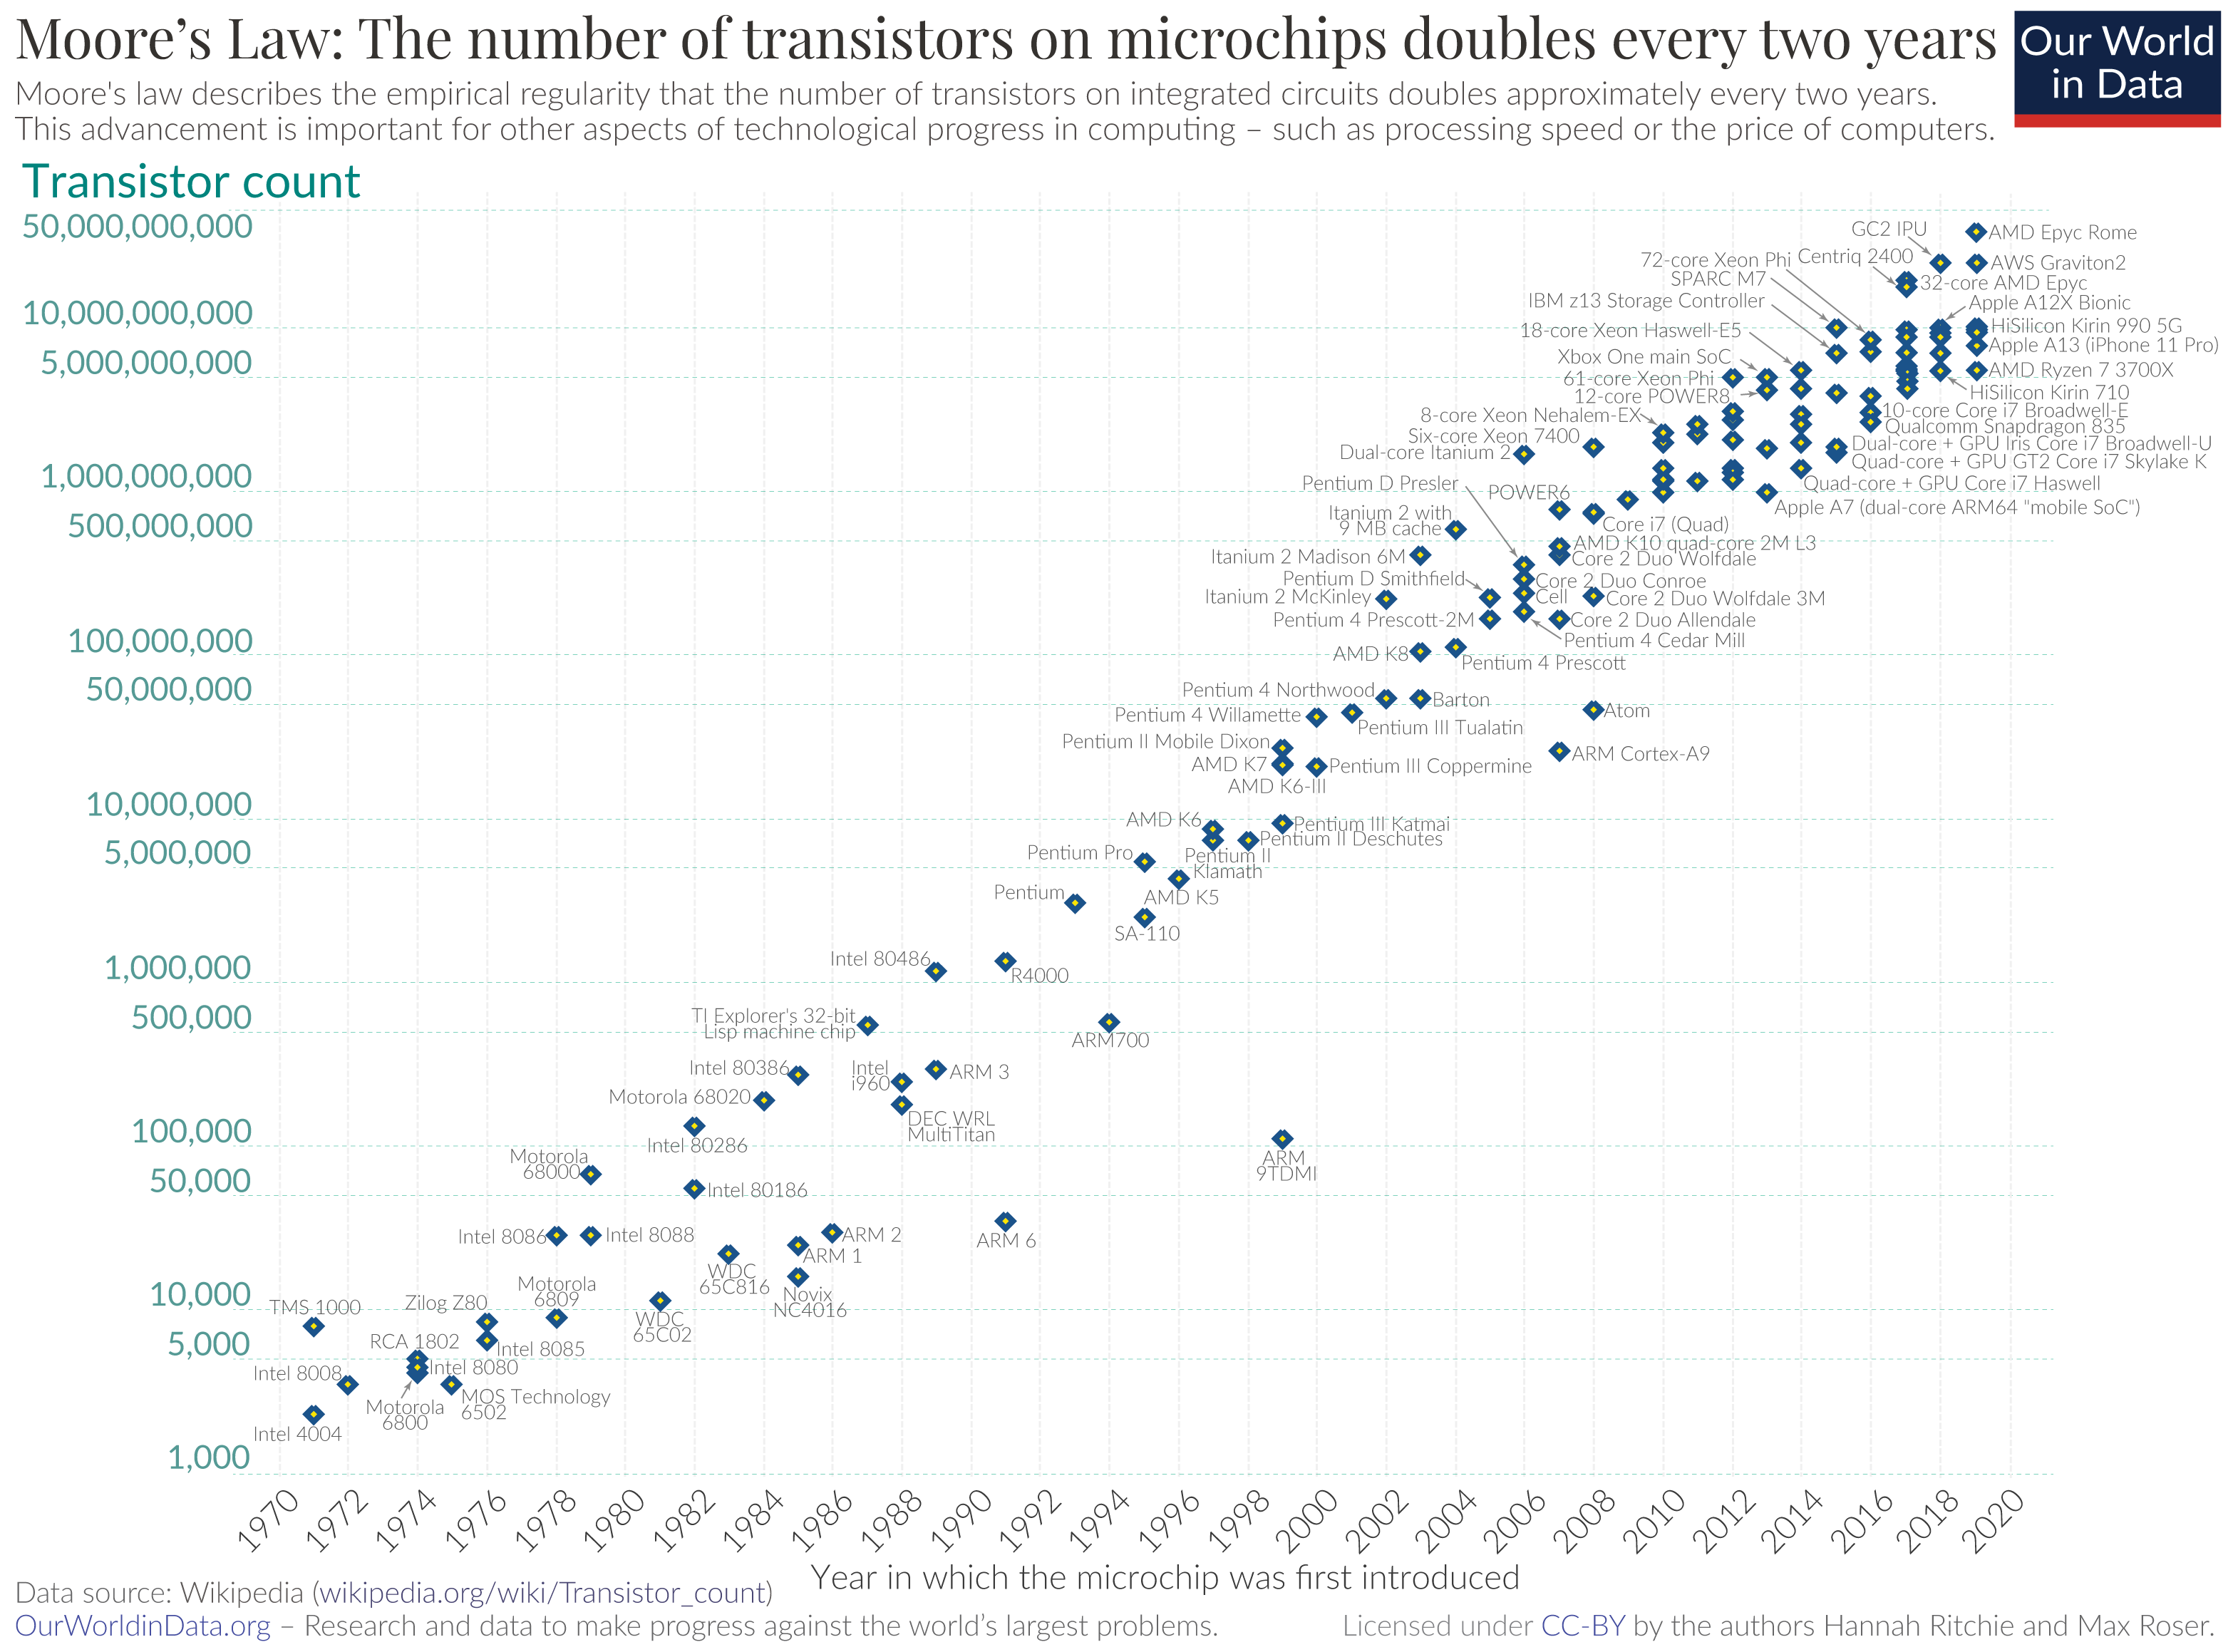
\includegraphics[width=70mm]{moore.png}}
\caption{Moore's Law.}\label{moore}
\end{figure}

\begin{figure}[!ht]
\centerline{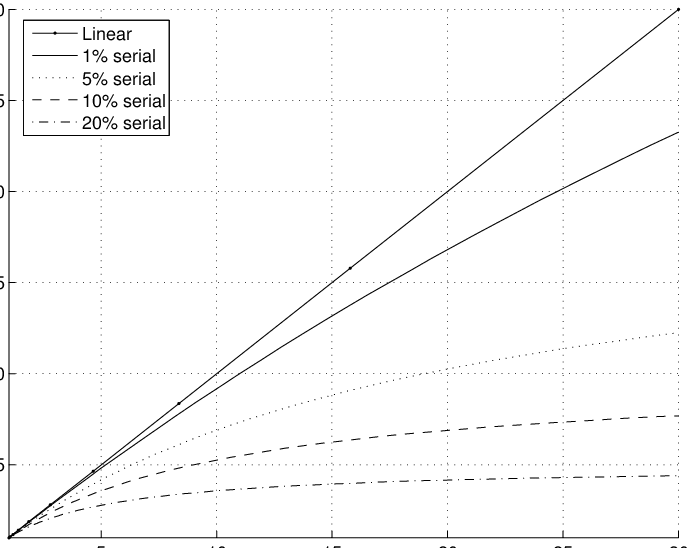
\includegraphics[width=70mm]{amdahl.png}}
\caption{Amdahl's Law}
\label{amdahl}
\end{figure}

With all this in mind, it becomes clear that the burden of increasing the performances of software no longer lies in the hand of hardware manufacturers, but rather on the hands of software engineers, who should attempt to have as little sequential code as they can in their programs.
Historically, it was the responsibility of the end programmer to parallelise their program. But there has been work to hide this work in the lower levels of the software stack \cite{scalable}, to make the shift from sequential to parrallel transparent to the higher levels. The scope of this work is at a lower level. The goal is to provide perfectly linearly scalable implementations of classic data structures, keeping the exact same interfaces, such that there could be virtually no modification to applications' source, while achieving the scalability that we desire.


\subsection{Work}
This project is a part of a bigger project around \textit{Degradable Data Structures}. These structures will be explained in more detail further in this paper. Simply put, these data structures are created by tweeking the specifications of classical data structures, in order to be able to change their implementations to better ones allowing for better scalability or performance. The idea is to take real industrial code, and change some of the objects used for degraded ones whithout having to change any of the code, and observe the increase in performance.

\subsection{Scope of this project}
The work being done here is the applications of these degraded data structures to a data store : Apache Ignite \cite{ignite}. We first need to locate situations in the source of the data store where it is judicious to apply degradation. This is done by benchmarking the application, and pinpointing the source of eventual bottlenecks, then figuring out whether or not degradation is possible.

\subsection{Contributions}
This project made the following contributions to Apache Ignite:
\begin{itemize}
  \item Benchmarking
  \item Perfomance Analysis
  \item Identification of bottlenecks
  \item Method for fiding the probable causes of bottlenecks
\end{itemize}

\subsection{Outline}
The rest of this paper details to context and the contributions of the project.

We shall start by examinating the related works and how they compare to the work being done here.

We will then explain the theory behind degradable objects and how we can find places to apply them.

We next will detail the information we gathered by analysing Apache Ignite.

we will then show the result obtained.

We will finally discuss the conclusions we can take from the work.


\section{Related Work}
\subsection{The Scalable Commutativity rule}
The approach of Austin Clements \cite{scalable} team is very similar to the work being done here. They present a new way of designing scalable and performant software, by thinking on the interface rather than on the implementation. They present the \textit{Scalable Commutativity Rule} that states that \textit{whenever interface operations commute, they can be implemented in a way that scales}. To describe this commutativity they provide a new definition calles \textit{SIM-Commutativity} for more complex interfaces. The idea is then to modify the interfaces so that the operations are commutative. This relates very much to the idea of degraded data structures, as they are an extension of this work : rather than saying that the interface needs to be modified, the idea with degradation is to remove some constraints of the previous interface, so that it scales. It could use commutativity or some other form of contraint on the interface.

In the scalable commutativity rule, they work on the interface of the linux kernel, whereas this work is more geared towards data stores and their data structures.

\section{Degradable Data Structures}
The goal of this project is to improve the performances of Apache Ignite, by inserting existing degraded data structures in the place of traditional data structures. We wil therefore first explain to what extent the implementation of data structures is linked with performance of parallel applications. We shall then explain the principle behind the degrading of objects, and we will finally explain how we can find the places where it makes sense to apply this degradation.

\subsection{Contention and Scalability} 
The relationship between the implementation of data structures and the performances of parallel applications is not immediate.

To achieve the best performance possible with parallel software, we need for it to scale. Meaning that increasing the number of parallel workers will increase the speed of the computation propotionally. As we have seen with Amdahl's Law, to do this, we need to have as little sequential code as possible in our program. One big source of sequentialness in software is contention in data accesses. Indeed, when two process try to access and modify the same data point at the same time, the result is non deterministic, which is really bad. To prevent this, safety measures are put in place to prevent concurrent accesses to the same piece of data. Often times, this results in the fact that only one process at a time can access the data, which we will call a \textbf{bottleneck}. This introduces sequentialness, and thus we loose in scalability.

We can therefore conclude that the goal of the designer of data structures is to prevent bottlenecks by avoiding contention on the same data points as much as possible, we call this \textit{conflict-freedom}

\subsection{What are Degradable Data Structures ?}
Many libraries provide really performant and scalable implementation of classical data structures for concurrent programming, for example,  the Java.Util.Concurrent library \cite{java_concurrent} provides wait-free and linearizable objects. However, the efficiency of these implementations are somewhat limited in a lot of situations, as they are supposed to respect to the letter the specifications (interfaces) of the data structures. Most of the time, these specifications are not designed with performance in mind, rather ease-of-use or generalizability. For example, a classical implementation of a counter needs the increment operation to return the value of the counter. There might be some situations when all these constraints are not necessary, and we loose in performance for nothing.

The idea behind degradation is to remove some constraints these specifications when they are not necessary. In the example of the counter for instance, if we say that we do not need for the increment operation to return the value, we can implement the object in such a way that the increment operation only updates a local value to the thread, and we gather the values only when the read operation is called. This would render the increment operation perfectly scalable, and thus really performant.

This is one example of how we can degrade an object, but there are many other solutions, and the work being done right now is to generalize this idea, and formalize it. A key insight is that operations can be implemented in a conflict-free manner, and thus scale, when their permutation is indistinguishable for future operations. This is an extension of the idea of commutativity from Austin Clements et al. \cite{scalable}. This can be understood quite intuitively : if the order of operations matters little, they can be applied locally and gathered whenever, thus ensuring conflict-freedom.

\subsection{How do we find where to apply degradation ?}


\section{Performance Analysis of Apache Ignite}

\section{Performance Evaluation}

\section{Conclusions}




\begin{thebibliography}{00}
\bibitem{scalable} \href{https://dl.acm.org/doi/10.1145/2699681}{Austin T. Clements, M. Frans Kaashoek, Nickolai Zeldovich, Robert T. Morris, and Eddie Kohler. 2015. The scalable commutativity rule: Designing scalable software for multicore processors. ACM Trans. Comput. Syst. 32, 4, Article 10 (January 2015), 47 pages.}
\bibitem{ignite} \href{https://ignite.apache.org/docs/latest/}{Apache Ignite}
\bibitem{gcpcompute} \href{https://cloud.google.com/compute/docs}{Google Cloud Platform Compute Engine}
\bibitem{moore} \href{https://ieeexplore.ieee.org/document/591665}{R. R. Schaller, "Moore's law: past, present and future," in IEEE Spectrum, vol. 34, no. 6, pp. 52-59, June 1997, doi: 10.1109/6.591665.}
\bibitem{amdahl} \href{https://conservancy.umn.edu/handle/11299/104341}{Gene M. Amdahl (1989), Oral history interview with Gene M. Amdahl, Charles Babbage Institute, University of Minnesota, hdl:11299/104341.}
\bibitem{java_concurrent} \href{https://docs.oracle.com/javase/8/docs/api/index.html?java/util/concurrent/package-summary.html}{Java.Util.Concurrent}

\end{thebibliography}

\vspace{12pt}
\end{document}
